\documentclass[12pt, fleqn]{article}
\usepackage[british,UKenglish]{babel}
\usepackage[utf8]{inputenc}

% Layout packages
\usepackage[
    a4paper,
    right=25mm,
    left=25mm,
    top=25mm,
    bottom=25mm,
    headheight=15pt
]{geometry}
\usepackage{fancyhdr} % Adds page headers with chapter info
\usepackage[justification=centering]{caption}
\usepackage[all]{nowidow} % Prevents orphans and widows (single lines at start/end of a page)
\usepackage{lscape} % For landscape-oriented pages (e.g. large figures)
\usepackage[nottoc]{tocbibind} % Includes bibliography in ToC
\usepackage{todonotes} % \todo and \missingfigure commands

% Table setup
% \usepackage{rotating}
% \usepackage{tabularx}
% \usepackage{booktabs}
% \usepackage{csvsimple}
% \usepackage{array}
% \usepackage{makecell}
% \usepackage{multirow}
% \renewcommand\theadalign{cc}
% \renewcommand\theadfont{\bfseries}
% \renewcommand\theadgape{\Gape[4pt]}
% \renewcommand\cellgape{\Gape[2pt]}
% \renewcommand{\arraystretch}{1.5}
% \newcolumntype{P}[1]{>{\centering\arraybackslash}p{#1}}
% \newcolumntype{Y}{>{\centering\arraybackslash}X}

% Graphics packages
\usepackage{graphicx}
\usepackage{pgfplotstable}
\usepackage{subcaption}
\graphicspath{{../img/}} % Sets root directory for image files
\pgfplotsset{compat=1.6}

% Maths packages
\usepackage{amsmath}
\usepackage[binary-units=true]{siunitx}
\sisetup{exponent-to-prefix=true, zero-decimal-to-integer}
% Hack to fix layout of sqrt with exponents:
% \usepackage{letltxmacro}
% \LetLtxMacro{\oldsqrt}{\sqrt}
% \renewcommand{\sqrt}[2][\mkern8mu]{\mkern-4mu\mathop{\oldsqrt[#1]{#2}}}

% Code listings packages, including syntax highlighting for Python
% (probably not needed for interim report)
% \usepackage{listings}
% \usepackage{xcolor}
% \definecolor{codegreen}{rgb}{0, 0.6, 0}
% \definecolor{codeblue}{rgb}{0, 0, 0.6}
% \definecolor{codegrey}{rgb}{0.4, 0.4, 0.4}
% \definecolor{codebrown}{rgb}{0.5, 0, 0}
% \lstdefinestyle{pystyle}{
%     basicstyle=\small\ttfamily,
%     language=Python,
%     commentstyle=\color{codegreen},
%     keywordstyle=\color{codeblue},
%     numberstyle=\tiny\color{codegrey},
%     stringstyle=\color{codebrown},
%     breakatwhitespace=false,
%     breaklines=true,
%     showstringspaces=false,
%     captionpos=b,
%     numbers=left,
%     numbersep=10pt
% }
% \usepackage{textcomp}
% \usepackage[T1]{fontenc}
% \lstset{
%     style=pystyle,
%     upquote=true,
%     columns=fullflexible,
%     keepspaces=true,
%     showlines=true
% }
% \renewcommand{\lstlistlistingname}{List of Code Listings}

% Typographical packages
\usepackage{setspace}
\onehalfspacing{} % Line spacing 1.5
\usepackage{nth} % \nth{3} compiles to 3rd, etc.
\usepackage[hidelinks]{hyperref} % Add clickable cross-references/hyperlinks in PDF
\usepackage{csquotes} % Context-sensitive quote marks, required by babel

% Hyphen issues
\pretolerance=10000 % Set to 500 for some hyphenation
\tolerance=2000
\emergencystretch=10pt


\begin{document}

    \pagestyle{empty}
    \hypersetup{pageanchor=false}
    \pagenumbering{alph}
    % !TEX root = ../report.tex

\title{CRUES Interim Report}
\author{Peter De Jonckheere, R. David Dunphy, Andrew Fagan, Matthew Gaffney,
Kyle Miller\\University of Strathclyde, Glasgow}
\date{\today}

\newgeometry{
    right=52mm,
    left=52mm,
    top=50mm,
    bottom=45mm
}
\thispagestyle{empty}
\begin{center}

    \LARGE
    Co-operative Robotics\\Using Environmental Sensors

    \vspace{1.5cm}

    \large
    -- 19520 Interim Report --

    \vspace{1.5cm}

    \textbf{Peter De Jonckheere, R. David Dunphy,\\Andrew Fagan,
        Matthew Gaffney,\\Kyle Miller}

    \vspace{0.3cm}

    University of Strathclyde, Glasgow

    \vspace{2cm}
    
\includegraphics[width=0.5\textwidth]{strath.png}

    \vfill{}

    \normalsize
    Proposer: Dr John Levine\\
    Supervisor: Dr Marilyn Lennon\\
    \today

\end{center}
\restoregeometry{}

    \pagenumbering{arabic}
    % !TEX root = ../report.tex

\begin{abstract}
\noindent This project aims to develop co-operative robotic systems which effectively map and search an area using non-telemetric sensors and communication. This will allow the systems to perform in environments which hinder telemetry, such as caves or tunnels.  Each robot should be able to solve this problem individually; however, after the introduction of multiple robots to the area, they should be able coordinate their movements to distribute the task and solve the problem faster. The robots will be tested in a custom-made testing environment---likely taking the form of a simple maze with a target that must be located---and evaluated based on their performance both individually and co-operatively.

Detailed analysis of the electrical, software and mechanical design solutions are presented. The robots will use a differential drive system and will be designed and constructed with the necessary hardware to complete the task of exploring their maze-like environment in a distributed fashion. Computer vision systems on the robots will be used in conjunction with ultrasonic sensors to perceive the environment and identify other robots in the group, and incremental encoders and an inertial measurement unit will be used to track the robots position and orientation. Communication will be conducted over either Wi-Fi or Bluetooth systems, which will be artificially restricted to require line-of-sight, so as to simulate situations where global communication is not possible.

The report also contains extensive discussion of the project management approach used to properly coordinate the project team. The structure of the team and practices employed have been considered carefully and a detailed timeline developed to limit project risk.

\end{abstract}

    % % !TEX root = ../report.tex

\renewcommand{\abstractname}{Acknowledgements}
\begin{abstract}
\setcounter{page}{2}
\centering
The authors would like to thank Drs. John Levine and Marilyn Lennon for the opportunity to work on such an interesting project, and the support throughout it, respectively. Thanks also to Steven Cartwright, whose constant help and advice with the project cannot be overstated. The authors would also like to thank friends and family who provided proof reading and moral support. Finally, a heartfelt thanks to Don Eskridge, who divided or united the team depending on the hour of the day.
\end{abstract}

    \hypersetup{pageanchor=true}

    \pagestyle{plain}
    \tableofcontents{}
    \clearpage{}

    \pagestyle{fancy}
    % !TEX root = ../report.tex

\chapter{Introduction}\label{introduction}
\section{Context}\label{introduction/context}
Using multiple co-operating robots (named and referred to as Blinky, Inky
and Clyde) can be a useful strategy when attempting to complete tasks that
can be divided and parallelised, such as exploration of a large area.
Usually, this requires a centralised control system that can
coordinate the robots to accomplish the task. However, in
environments where radio communication is impossible or severely restricted,
such as underground or in areas with high interference, these systems would
be unable to complete their task. In these circumstances, communication may
be limited to non-telemetric sensors that require line-of-sight. Therefore,
intelligent systems are required so they can co-operate effectively.

Co-operative robotics can be used to solve a variety of tasks more 
effectively than a more complex individual robot, introducing distribution
and redundancy into the system which can be highly advantageous over single 
agent systems~\cite{dudek96}. This redundancy can be mission critical in 
scenarios where a hazardous environment poses risks to individual robots. 
Therfore the loss of any single robot is not fatal to the mission as all
the robots are homogenous and can can complete the task individually.

Previous research into co-operative robotics has focused on UAVs~\cite{khan18},
non-autonomous agents~\cite{jimenez18}, or made use of extensive
communication, such as by using the cloud~\cite{wensing2018cooperative}.
This study will use restricted non-telemetric communication (i.e. local 
communication between neighbouring robots rather than communication over a 
central server). Co-operating effectively under this limitation poses
additional challenges, which need to be overcome to allow
collaborative robotic exploration of environments such as caves. This
application area was inspired in part by a recent incident necessitating cave 
exploration and rescue in Thailand~\cite{bbcthailand}.

In order to remove the physical complexities of operating on difficult
terrain and allow research to focus on communication and problem-solving 
algorithms, a toy problem has been devised for the robots to solve. This
will take the form of a simple maze which contains a target that needs to
be found and identified by the robots. The primary aim of the study is to
construct multiple robots which can navigate this maze and co-ordinate their
efforts to find the target more quickly than could be achieved by each robot 
individually.

An additional requirement is that the robots should be constructed using
inexpensive components. This is necessitated by the increased cost implied
by the need for multiple robots, in addition to mitigating the risk in the 
event of the robot failure given the potentially dangerous environments.

\section{Objectives}\label{introduction/objectives}
\begin{itemize}
\item{Design a simple differential drive robot capable of exploring and perceiving its environment---Major Objective}
    \item{Construct two robots using this design---Major Objective}
    \item{Develop a Simultaneous Localisation and Mapping (SLAM) algorithm to allow the robots to explore an area---Major Objective}
    \item{Develop a system to allow the robots to interact and communicate with each other---Major Objective}
    \item{Develop algorithms to search a maze which can be dynamically parallelised over any number of agents---Major Objective}
    \item{Develop a test environment and evaluate the robots’ performance---Major Objective}
    \item{Add additional robot(s) and evaluate scalability of approach---Optional Objective}
    \item{Improve SLAM by adding loop closure between robots---Optional Objective}
\end{itemize}

    % !TEX root = ../report.tex

\chapter{Background}\label{litreview}

\section{Co-operative Robotics}\label{litreview/robotics}
A robot is ``a machine capable of carrying out a complex series of actions 
automatically''~\cite{robotdef} and robotics is the ``branch of technology which deals with the design, construction, 
operation, and application''~\cite{roboticsdef} of robots. Robotics combines a number of fields from mechanical,
electrical and software engineering within a single system to achieve its goals. By 
combining the three major disciplines of artificial intelligence, operations 
research, and control theory, a resultant intelligent control system is created~\cite{saridis1983intelligent} which can be 
used for a wide range of robotic applications.

Co-operative robotics has varied definitions across different papers. One such
definition, which generalises co-operative behaviour in robotics, describes it 
as ``joint collaborative behaviour that is directed toward some goal in which 
there is a common interest or reward''~\cite{barnes1991behaviour}. This 
description fits the objectives of this study more appropriately than the 
specific term ``swarm robotics'',  which has a number of additional requirements, 
including that problem solving should be distributed across the swarm~\cite{sahin04}. This definition does not apply to this project, as the robots 
designed herein are capable of operating autonomously and will be able to solve 
certain tasks individually. In this case, collaboration is used to deliver a 
performance improvement. For this reason, the more general term of co-operative 
robotics will be used throughout. 

The aim of co-operative robotics is to reduce the time taken or 
increase performance  of the system over a single-robot system~
\cite{premvuti1990consideration}. Additionally, by creating a decentralised and 
distributed system across several homogeneous agents, agent redundancy is 
introduced which can improve the completion rate of tasks, especially in 
potentially volatile environments~\cite{beckers1994local, parker95}.
Co-operative robotics goes beyond the idea of collaborative robotics in 
requiring an additional aspect of intelligence in the communication and 
coordination of the individual agents~\cite{cao1995cooperative}. 

Co-operative robotics is an area of active research, and is growing in popularity --- as the
capabilities of the technology increases --- as it can be used in a wide-variety of
situations. In 2011, co-operative robotics was used as part of the
response to the Great Eastern Japan Earthquake. A team from Kyoto University
used co-operating, remotely operated, underwater vehicles to search for submerged
debris to assist with resuming fishing in the region~\cite{matsuno2014utilization}.
Although co-operative, their systems still required a level of human control.
Dr Nithin Mathews' research in 2012 provided a communication system without
human interaction~\cite{mathews2012spatially}. This allowed many smaller robots
to co-ordinate to complete tasks that one could not on its own, such as push a
larger object. Their system, however, requires a global view of the area to 
co-ordinate their efforts. However, even since these findings, the progress
in the field has accelerated. An excellent example is Sebastien de Rivas' work at
Harvard University~\cite{rollsroyceSWARM}. In partnership with Rolls Royce, his
team have spent the last eight years developing very lightweight co-operating robots.
Currently, weighing \SI{1.5}{\g} and measuring \SI{4.5}{\cm} in length, the
four-legged micro-robots have eight degrees of freedom, and are being developed with
the aim of reducing their size so they can inspect the internal workings of an engine.

\section{Robotic Control} \label{litreview/robotics/control}  
As the robots in this study are homogeneous and should be able to complete 
tasks individually, control is limited to the control of a single robot in the 
complete system. Robotic mechanisms form the control system for a robot and 
connect the fixed parts of the robot together by joints, allowing motion between 
these fixed parts~\cite{lynch2017modern}. Actuation of the joints, usually 
by motors, imparts forces on the robot which allow it to move and perform a 
variety of tasks~\cite{lynch2017modern}. The movement of these ``actuators'' 
is influenced by several sensors which provide the system with information 
about its environment. These sensors can also influence the movement of the 
actuators through feedback from previous movement instructions~\cite{lynch2017modern}.    

Sensors can take many forms and provide information about internal and external 
environmental factors of the robot. External sensors provide information which 
the robot would otherwise find significantly more difficult to discover, one 
such example being range sensing. This can take a number of different forms 
including ultrasound, infra-red, Light Detection And Ranging (LIDAR) and 
binocular computer vision. Each of these sensors use unique methods to determine 
the distance from the robot to another object in its environment. Ultrasound 
sensors use high frequency sound waves which reflect from surfaces and return 
to the sensor. The time taken to return and the speed of sound is used to 
calculate the distance to the object. Infrared sensors work in a similar 
fashion but with invisible light instead of sound. 

LIDAR is a more advanced use of invisible light to more accurately detect 
distance using more powerful and precise beams of light than in the infrared 
case~\cite{lidar}. Binocular vision allows depth perception to take place 
similar to that allowed by human vision~\cite{read2005early} by perspective-based cues~\cite{pfautz2002depth}. 

Internal sensors can either be related to the actuators or fixed parts of the 
robot. Those sensors which are connected to the fixed parts of the robot provide 
feedback about the entire robot and its local environment. The Inertial 
Measurement Unit (IMU) provides feedback regarding the acceleration and angular 
velocity with relation to 6 different axes (x, y, z in both linear and angular 
planes) or Degrees of Freedom (DOF). This can be combined with information from 
other sensors in order to reduce the overall error in determining the robot's 
location with relation to its starting position.  

One such sensor is the encoder which is connected to the wheels and provides 
only feedback information about this actuator. These sensors are connected 
directly to the shaft of the motors and provide the control system with the 
actual distance moved by the motors. This allows adjustments to be made and each 
of the wheels to be maintained at a constant speed when utilised by the 
Proportional-Integral-Derivative(PID) controller of a robot.  

\subsection{PID Controller}\label{litreview/robotics/pid}
As mentioned above, PID controllers are a very common solution to problems where the error of the 
system (the difference between the current state and the desired state) can be 
measured. Proportional-Integral-Derivative refers to the 
function of the error with which the output is calculated. The output of the 
system is the summation of a term which is proportional to the error, a term 
which is related to the error integrated over time, and a term which is 
proportional to the rate of change of the error~\cite{aastrom2006advanced}. This is shown by Equation \ref{eqn:pid}.

\begin{equation}
\label{eqn:pid}
O(t) = k_{p}e(t) + k_i\int_{0}^{t}e(t)dt + k_d \frac{\mathrm{d} e(t) }{\mathrm{d} t}
\end{equation}

If $K_d$ and $K_i$ were both 0, and only the P term was active, the output 
would change to reduce the error in the system. For example, with a
temperature controller, if the temperature was too low the heater would
turn on, with the difference between the actual temperature and the required 
temperature used to adjust how high it was set. In many systems, this simple 
implementation is adequate, however it has several limitations. 

Consider for instance the temperature controller example where heat is being
lost in the system is equal to the P constant times the error. This would
result in a stable state with a potentially large error. To prevent this,
the I term can be increased. This will increase the longer an error is
present, thus preventing stable state errors. 

Again, PI controllers are a common control mechanism, however they often have 
a problem with overshoot due to system inertia. Once more considering the 
temperature controller, this is where the heater is set to increase the 
temperature, and the desired temperature is reached. The heater turns off, but 
is still hotter than the rest of the system, causing the system to get too hot. 
This is especially damaging in systems where the control in one direction 
is passive, e.g. the system can actively heat up, but must wait for heat loss 
to cool down. This problem can be mitigated by increasing the D component. 
This will push the state towards the desired state when the error is increasing 
(e.g. during over-shoot), and pushes the current state away from the desired 
state as the error is reducing as to minimise overshoot before it 
occurs. This does, however, reduce the response speed of the system~\cite{chen2007linear}.

One method of tuning a PID controller is the Ziegler-Nichols method~\cite{ziegler1942optimum}. This principle originates from before autonomous 
robotic control and has been adapted for this application~\cite{aastrom2004revisiting}. The method experimentally finds the critical gain 
of $K_p$, $K_u$, from which the frequency of oscillation, $T_u$ can be found. 
These values can then be used to calculate $K_i$ and $K_d$ which results in a 
tuned system. However, many different formulae and definitions of the critical 
gain of $K_p$ exist in literature. This leads to the conclusion that the 
Ziegler-Nichols method is mathematically imperfect, and this will have to be 
explored experimentally during the project.

\section{SLAM}\label{litreview/slam}
A key challenge in mobile robotics is for the robot to know its own position in the
environment whilst still being able to build a map of its surroundings. 
This is especially true in the absence of external referencing systems
such as GPS to aid in knowing its relative position. This is known as the Simultaneous Localisation And Mapping (SLAM)
problem and has been one of the most extensively researched topics in mobile
robotics over the last two decades~\cite{grisetti2010tutorial}. As the robot's
estimate of its position is affected by both the previous state's uncertainty
and any errors in the current measurement, the uncertainties compound
over time. To rectify this, a map with distinctive landmarks can reduce its
localisation error by revisiting these known areas. This is known as loop closure.

SLAM implementations rely on sensor fusion algorithms as part of their implementation. 
These take in readings from an array of sensors and calculate an estimated state change
based on the probability of error for each sensor. This effectively allows errors between 
multiple sensors to be cancelled out, resulting in more reliable estimates. A standard 
approach is to use sensor fusion to combine odometry readings from wheel encoders with 
acceleration information obtained from an inertial measurement unit (IMU) to correct for 
errors caused by wheels slipping and sensor imperfections.

There are a large variety of solutions to suit various system requirements, these
can be categorized as either filtering and smoothing. Filtering creates a state estimation 
using the current robot position and the map. The estimate is augmented and improved
by using the new measurements as they become available. Some popular
approaches to filtering are techniques such as Kalman filters, particle filters
and information filters. Smoothing techniques involve a full estimate of the trajectory of
the robot from all available measurements. These typically use least-square error 
minimisation techniques and are used to address the problem known as the full SLAM 
problem which attempts to map the entire path.

The state of the system is known as $x_k$ which is a function that uses the previous 
state to determine the next state. As this can not be perfectly accurate, there will 
be uncertainty in the readings that must be considered. As a result, $x_k$,
which is known as the motion model, is defined as
\begin{equation}
x_{k} = f(x_{k-1}, q_{k-1})\,,
\end{equation}
where $q_{k-1}$ is the randomness introduced to the system. As such, this can
also be represented by the probability distribution
\begin{equation}
x_{k} \sim p(x_{k} | x_{k-1})\,.
\end{equation}
Both equations imply that the state is stochastic and depends on the previous
state. The probability distribution emphasises that the current state is
drawn from a distribution of possible states based on the previous state. Given that a perfect sensor is not possible, the current state will also have noise
in the reading. This is known as the measurement model and can be defined as
\begin{equation}
y_{k} = h(x_{k}, r_{k})\,,
\end{equation}
where $r$ represents the uncertainty of the sensor. As
before this can be expressed as an uncertainty model:
\begin{equation}
y_{k} \sim p(y_{k} | y_{k-1})\,.
\end{equation}
It is assumed that the motion and measurement models are Markovian in that
the current state only depends on the previous state. The measurement model only
depends on the current state and no previous values.

By applying Bayes' theorem and marginalisation the current state can be described as
\begin{align}
\label{eqn:predict}
p(x_{k} | y_{1:k-1}) & = \int p(x_{k}|x_{k-1}) p(x_{k-1} | y_{1:k-1}) dx_{k-1} \\
\label{eqn:update}
p(x_{k} | y_{1:k}) &= \frac{ p(y_{k}|x_{k})p(x_{k}|x_{1:k-1})}{ p(y_{k}|y_{1:k-1})}\,.
\end{align}
Equation~\ref{eqn:predict} is known as the predict equation. By integrating over
the previous state, all potential outcomes of the state $x_k$ are
considered. Equation~\ref{eqn:update} is referred to as the update equation,
as the prediction is updated using the new measurement information~\cite{kam1997sensorfusion}.

One of the most common methods of implementing SLAM is filtering using an
Extended Kalman Filter (EKF). An EKF is an efficient, recursive filter
that estimates the state of a dynamic system from a series of noisy measurements~\cite{fox2003bayesian}.
This uses the premise of the predict and update equations as joint probability
distributions. Given variables defined on a probability space, the joint
probability distribution gives the probability that each of the variables falls in any
range or set. It uses these techniques to estimates a state vector containing
both the location of landmarks in the map and the robot pose~\cite{huang2007convergence}.


\section{Computer Vision}\label{litreview/cv}
Computer vision is the analysis of digital image or video frames to allow a computer
system to gain a high-level understanding of the 3D environment contained within
the image\cite{CVBallard}. A common application for computer vision is the identification and classification
of objects. Identification generally involves the recognition of features of the
object and the comparison of these features and their relative positions to a
known model of the object. Classification usually involves machine learning
algorithms to build up a definition of the object based on its visible properties\cite{CVpaoletti2018new}.

Computer vision can also be used to triangulate the position of objects in the
field of view by measuring the discrepancy in the object's position in the two camera
frames given a translation matrix relating the two cameras.

Computer vision can be well integrated with SLAM providing a means of both the measure
of distance (if the CV system is bi-ocular) and the identification of distinctive
features in the environment to allow loop closure\cite{CVho2006loop}.
\subsection{Object Detection}\label{litreview/cv/objDet}
\subsubsection{CNN}\label{litreview/cv/objDet/CNN}
A common method for object detection is to use a Convolutional 
Neural Network (CNN)~\cite{schmidhuber2015deep}. This is a deep learning method that 
considers the relative position of pixels in the image. It 
works by scanning a Locally Receptive Field (LRF) across the 
image, and searching this small group of pixels for patterns 
at each position as it moves. This results in a set of 
matrices of outputs, which can then be scanned again. With 
each iteration, the complexity of pattern which can be detected 
increases. The output of these convolutional layers is then 
pooled (combined to reduce size), and used as the input to a 
neural network which can then classify the image.


\subsubsection{Feature Based}\label{litreview/cv/objDet/fb}
Another approach to object detection is feature based. This 
involves the identification and comparison of key points in an 
image of the target object and in the camera frame~\cite{lowe2004distinctive}. There are 
several key point detection algorithms --- SIFT, BRISK and ORB, 
to name a few --- each of which has its own way of describing 
patterns in the pixels and selecting which will be rarer and 
therefore, more useful when identifying objects. Each also has 
a method of quantifying the similarity of two matches called a 
distance metric. The algorithm then looks for features in both 
the frame and the object image which score low in the distance 
metric (indicating similarity), filters the matches to remove 
false positives, and then uses the relative positions of the 
matches to estimate an outline of the object in the image 
frame. 

\section{ROS}\label{litreview/ROS}
The Robot Operating System (ROS) is a framework for developing robot
software designed to allow flexible software design. It is a collection of tools, 
libraries and conventions that aim to simplify creating complex and robust robotic systems across a variety of platforms~\cite{aboutROS}. 
It was designed with the objective of being as modular and distributed
as possible. This modularity allows the user to be able to use as much or
as little of ROS as they desire, where their own implementation can be
easily fit into the system~\cite{rosForMe}.

ROS uses a peer-to-peer networking topology to allow communication 
throughout the system. These systems consist of a number of processes  
that perform the system's computation called nodes which can  
run across multiple machines. The peer-to-peer topology requires 
a lookup mechanism to allow processes to find other process' addresses at 
runtime so they can communicate. Nodes communicate by passing messages 
that are data structures of typed fields which can include arbitrarily nested 
structures and arrays~\cite{crick2017rosbridge}.


Nodes can use two distinct ROS frameworks, services and topics. 
Services are synchronous and perform like function
calls in traditional programming languages, where only one node in the 
system can provide a service of a specific name. Alternatively, topics are
asynchronous streams of objects published by a node. Other nodes can 
subscribe by creating a handler function when a new data object is available.
Multiple nodes can concurrently publish and/or subscribe to the same topic and
a single node may publish and/or subscribe to multiple topics.

ROS was also designed to be language-neutral and supports languages 
such as C++, Python and Octave. To support this cross-language 
development, ROS uses a simple, language-neutral Interface Definition 
Language (IDL) to describe the messages sent between modules 
\cite{quigley2009ros}. Code generators for each language then generate 
native implementations which are serialised and de-serialised by ROS 
as messages are sent and received. This results in a language-neutral 
message processing scheme where languages can be used as the programmer 
prefers based on the requirements of that given module. 

There are other alternatives to ROS, such as Yet Another Robot Platform 
(YARP). YARP was designed to attempt to make robot software more stable 
and long-lasting without compromising flexibility to change the sensors, 
processors and actuators. It also communicates using a peer-to-peer 
topology with an extensible family of connection types however, YARP is 
written in C++ and does not support other languages \cite{aboutYARP}.
The YARP model of communication is transport-neutral, meaning the details 
of the underlying networks and protocols in use are decoupled from the 
data flow \cite{exactlyIsYARP}. Compared to ROS, YARP is less widely used.
As a result, it does not have the same extensive range of libraries available 
which implement commonly required functionality for a robotic system.

\section{AI}\label{litreview/maze}
Artificial intelligence is another component of intelligent robotic control and is the 
development of computer systems able to perform tasks normally requiring human intelligence~
\cite{russell2016artificial}. Searching problems, and the algorithms which solve them, are a 
common branch of artificial intelligence, into which much research has been undertaken. Search 
algorithms and optimisation algorithms can be thought of as highly similar, and in the case of 
a weighted tree search, which maze exploration can be modelled as, either can be used to solve the problem~\cite{kanal2012search}. 

\subsection{Maze Exploration}\label{litreview/maze/exploration}
The exploration of an unknown environment is a well-researched problem in 
robotics. Robot exploration is particularly important for 
environments that are difficult or dangerous for humans. There are many
algorithms that can be used for exploration such as Wall Follower, 
Trémaux's and Pledge.

One of the simplest exploration algorithms is the Wall Follower algorithm, 
also known as the right-hand rule, when prioritising turning right, or 
left-hand rule, when prioritising turning left. If the maze is simply 
connected, that is there are no loops in the maze, then the Wall Follower 
algorithm is guaranteed to reach a goal/exit if one exists. Otherwise, the 
algorithm will return to the starting point having traversed every corridor at 
least once~\cite{wallFollowerArcBotics}. The steps of the algorithm are 
relatively straightforward. The right-hand rule algorithm is shown in Algorithm~\ref{alg:wf}. 

\begin{algorithm}\label{alg:wf}
\caption{Wall Follower Algorithm}
\begin{algorithmic}
\REPEAT
\IF{robot can turn right}
  \STATE turn right
\ELSIF{robot can go straight on}
  \STATE go straight on
\ELSIF{robot can turn left}
  \STATE turn left
\ELSE
  \STATE dead end reached, turn 
\ENDIF
\UNTIL{goal is reached}

\end{algorithmic}
\end{algorithm}

These steps ensure to keep a wall on the right hand side of the robot at 
all times. The left-rule is just the opposite where the robot turns left 
if possible to keep the wall on the robots' left. Therefore,
this algorithm is inherently inefficiently as it exhaustively searches the
maze. In many cases, one of these algorithms would be significantly quicker
than the other but which cannot be determined without prior knowledge of 
the maze.

An alternative to the Wall Follower algorithm is Pledge's algorithm. This
aims to solve the problem where Wall Follower could be stuck in a loop. An 
example of which is: if walls form to create a rectangle in the centre of 
the maze, the robot would continually turn right or left (depending on
algorithm) around that rectangle, never finding the exit. Pledge solves this
by keeping a count of the number of turns made (if not right-angled turns,
then the angle of turn is used instead) as well as the initial direction of
travel. \cite{klein2011pledge}

\begin{algorithm}
\caption{Pledge's Algorithm}
\begin{algorithmic}
\STATE Set angle counter to 0
\REPEAT
\REPEAT
\STATE Walk straight ahead;
\UNTIL {wall hit};
\STATE Turn right;
\REPEAT
\STATE Follow the obstacle's wall;
\UNTIL{angle counter = 0;}
\UNTIL {exit found;}
\end{algorithmic}
\end{algorithm}

Using the initial direction and counting the turns made, allows the 
algorithm to avoid traps such as loops which simple wall followers can be caught in, such as an approximate ``G'' or ``6'' shape.

The Trémaux maze-solving algorithm requires the robot to record its 
path and mark the routes it has taken throughout its navigation routine. Any 
given path can be unmarked, marked once or marked twice. If a path is marked 
twice that indicates the robot has travelled down it in both directions. The 
robot will not travel down any path marked twice for a third time, therefore 
treating them as dead-ends. Paths without markings are prioritised, before 
choosing those marked once in search of further unmarked paths. If a 
solution is found then the path that is marked only once is the route 
from the goal back to the start point. Otherwise if no solution is found,
all paths in the maze will be marked twice \cite{even2011graph}.
Importantly, this will likely not find the shortest path, but it will be 
guaranteed to find one if it exists.

\subsection{Path Finding}\label{litreview/maze/path}
There are many algorithms that can be used to find the shortest path 
through a graph such as Dijkstra's algorithm and A* search. In the 
context of our agents, path finding is likely to be used once 
the goal has been found to return the robot back to its starting 
position. In the case of an unweighted graph (a graph where all edges are 
equivalent to search), one of the simplest algorithms 
is breadth-first search. This explores all neighbours at the same depth 
before moving onto nodes at the next depth level. This would be guaranteed 
to find a path with the shortest number of edges and is $\mathcal{O}(|V| + |E|)$ 
where $|V|$ is the number of vertices and $|E|$ is the number of edges~\cite{cormen2009introduction}
Breadth-first search searches the oldest discovered node first meaning 
many backtracks are needed to reach the oldest discovered node. As 
backtracking in physical space is expensive, this results in a very 
costly search for a single-agent. As more agents are added, the cost of this 
decreases as less backtracking would take place. 

In the case where the edges have a weighting, which in our case would be the 
distance to next junction, Dijkstra's algorithm is one 
of the most commonly used methods for finding the length of shortest path between a specified pair of nodes in the graph. The steps for Dijkstra's algorithm are outlined in Algorithm \ref{alg:Djikstra}.

\begin{algorithm}
\caption{Dijkstra's Algorithm}
\label{alg:Djikstra}
\begin{algorithmic}
\REQUIRE{G = \{vs, es\} : G :: Graph, vs :: List(Vertex), es :: List(Edge)}
\REQUIRE{initial $\in$ vs : initial :: Vertex}
\REQUIRE{successors :: Vertex $\to$ List(Vertex); Finds vertices connected to input}
\REQUIRE{weight :: Edge $\to$ Int; Weighting factor applied to edge}
\REQUIRE{edge :: Vertex $\to$ Vertex $\to$ Edge; Finds edge which links vertices}
\FORALL{v $\in$ vs}
  \STATE{distance[v] $\gets \infty$}
  \STATE{visited[v] $\gets$ False}
\ENDFOR
\STATE {distance[initial] $\gets 0$}
\REPEAT
  \STATE{next $\gets$ v : distance[v] = min(distance) \AND visited[next] = False}
  \IF{no available next}
  	\RETURN distance
  \ENDIF
  \IF{distance[next] = $\infty$}
    \RETURN null
  \ENDIF
  
  \STATE{visited[next] $\gets$ True}
  \FORALL{v $\in$ successors(next) : visited[v] = False}
    \IF{distance[next] + weight(edge(next, v)) < distance[v]}
      \STATE{distance[v] = distance[next] + weight(edge(next, v))}
    \ENDIF
  \ENDFOR
  
\UNTIL{return condition reached}
\end{algorithmic}
\end{algorithm}

This version of Dijkstra's algorithm runs in $\mathcal{O}(|V|^{2})$ 
\cite{xu2007improved}. An improvement to this original algorithm using a 
min-priority queue implemented using a heap, runs in $\mathcal{O}
(|E| + |V|log |V|)$ and was first proposed in~\cite{fredman1987fibonacci}.


Developed initially as an extension of Dijkstra's algorithm, A* is a 
path-finding algorithm that typically achieves better performance by 
use of a heuristic. At each node, A* chooses the node which it believes 
can be used in the shortest path. It does so by choosing the node with 
the lowest value of f, where f is the sum of g and h, where g is the 
distance to the current node plus the known distance to that adjacent 
node and h is the heuristic value from that node to the goal. The heuristic 
value can be found exactly as the first step of the algorithm though 
this is very time consuming, so approximate heuristics are used such 
as the Manhattan distance, Diagonal distance and the Euclidean distance. 

    % !TEX root = ../report.tex

\chapter{Design}\label{design}

    % !TEX root = ../report.tex

\section{Project management}\label{plan}
\thispagestyle{plain}

\subsection{Project structure}\label{plan/structure}

At a high level, the project was structured as a team within a hypothetical
engineering consultancy being commissioned to undertake the project. This creates
several key roles both within and outside of the team, including a sponsor, a
supervisor, a project manager, and one or more consultants. The sponsor of the
project, Dr John Levine, provided the topic and the initial aims of the
project, but has no formal role in the project as it develops, except for
clarification of requirements and recommendations for design decisions.

The team supervisor, Dr Marilyn Lennon, serves as an advisor and manager of
the team, providing guidance in project management and general engineering
guidance, though without in-depth technical knowledge of the subject matter.
This role is very useful, as it enforces good engineering practices and
project structure, while preventing the project management from being
inhibited by details overly specific to the project.

Since the supervisor does not have all the technical knowledge the team
requires, other academics will take on the role of consultants, allowing the
team access to in-depth specialist knowledge. Examples of consultants who have
already contributed advice to the project are Dr Mark Post and Dr James Irvine,
who have supplied insight into practical robotics and microcontrollers,
respectively. This also has the benefit that,
while the team retains access to the expertise of the consultants, they are not
formally part of the project, so the team still has the final judgement in
design decisions.

Within the team, a project manager was appointed. The manager is not a team
leader, and has no increased authority over design decisions, but assigns tasks
and enforces deadlines on the whole team. This
attempts to ensure each team member is able to contribute to decisions made by
the group, and that all options are given equal consideration. It also imposes
order on the structure of the team while minimising needless bureaucracy.

\subsection{Project workflow}\label{plan/workflow}

All files relevant to the project are stored on a GitHub repository for
version control and access by all team members. The master branch cannot be
modified except by branch merging, so team members must work on their own
branches, and another team member must approve changes to allow them to be
finalised.

The repository is integrated with Slack, a tool for team communication.
Discussions are either held on Slack, or minutes are uploaded to Slack.
Tasks are created during meetings and posted as issues on GitHub immediately.
Each task is attributed to team members on a voluntary basis, and failing
that by assignment by the project manager.

\subsection{Objectives}\label{plan/objectives}

The specific objectives of this project were as follows:
\begin{itemize}
    \item{Design a simple differential drive robot capable of exploring and perceiving its environment---Major Objective (Source: Section~\ref{design/mechanical/conclusion})}
    \item{Construct two robots using this design---Major Objective (Source:~\ref{introduction/context})}
    \item{Develop SLAM algorithm to allow the robots to explore an area---Major Objective (Source: Section~\ref{design/software/conclusion})}
    \item{Develop a system to allow the robots to interact and communicate with each other---Major Objective (Source: Section~\ref{design/software/conclusion})}
    \item{Develop algorithms to search a maze which can be dynamically parallelised over any number of agents---Major Objective (Source: Section~\ref{design/software/conclusion})}
    \item{Develop a test environment and evaluate the robots’ performance---Major Objective (Source: Section~\ref{introduction/context})}
    \item{Add additional robot(s) and evaluate scalability of approach---Optional Objective(Source: Section~\ref{introduction/context})}
    \item{Improve SLAM by adding loop closure between robots---Optional Objective (Source: Section~\ref{background/slam})}
\end{itemize}

\subsection{Risk evaluation}\label{plan/riskeval}
The main technical risks of the project initially revolve around possible lead times for the ordering of parts. This will be mitigated by ordering parts as soon as feasibly possible and also by carrying out other work such as research and further design planning in the interim. Following on from this, components will also form the main aspect of technical risk in the latter stages of the project such as if a part is damaged or stops working. In order to mitigate this risk, time is left at the end of the project where no parts are being worked on directly and so it is unlikely for components to be broken. Time for testing, evaluation and report writing can also be used to order new components in serious cases. For components with extensive lead times in the first instance, spares may be ordered---if not too expensive---to further eliminate this risk.


\subsection{Timeline}\label{plan/timeline}

The Gantt chart here Figure~\ref{figure:gantt} was created using the objectives determined in each section of the design (Section~\ref{design}). The timescales were determined approximately using knowledge obtained from research with the addition of time for possible technical risks. These were considered carefully and an agile method was adopted in order to allow the tasks to be completed and give a small margin of error within the Gantt chart. For example, assembly of remaining robots is allocated a longer time than expected as this will involved lead times for components and also spans the period of time when the labs will be closed and construction work may not be possible.

Figure~\ref{figure:gantt} shows a Gantt chart of the project timeline.


\begin{landscape} % Rotates the image on the page
\global\pdfpageattr\expandafter{\the\pdfpageattr/Rotate 90} % Rotates the page in the PDF output
\begin{figure}[!p]\centering
    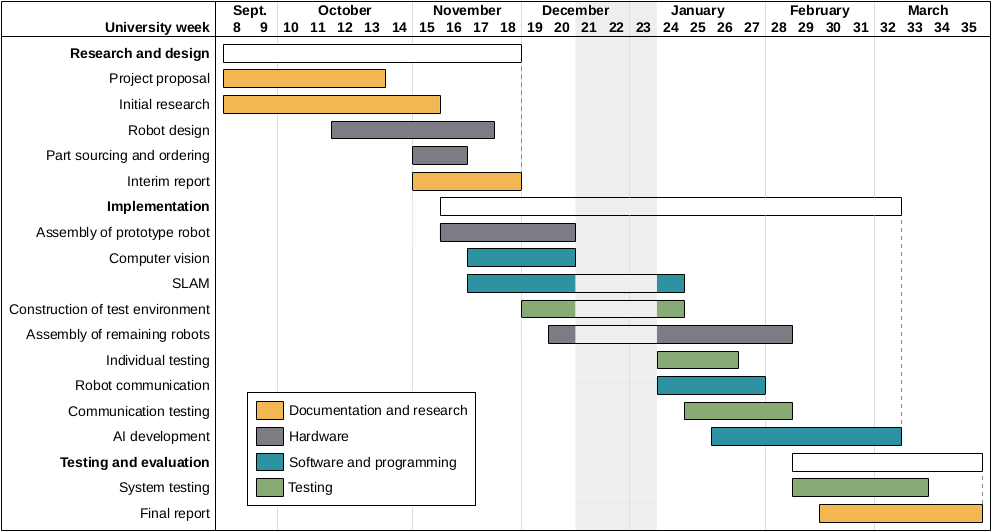
\includegraphics[width=1\linewidth]{gantt}
    \caption{Gantt chart}\label{figure:gantt}
\end{figure}
\end{landscape}
\global\pdfpageattr\expandafter{\the\pdfpageattr/Rotate 0}

    % !TEX root = ../report.tex

\chapter{Conclusion}\label{conclusion}


    \pagestyle{plain}
    \bibliographystyle{ieeetr}
    \bibliography{references}

    % \appendix{}
    % % !TEX root = ../report.tex

\chapter{Some stuff to go after the main report}\label{appendix/a}

The code for this project can be found at:
\begin{center}
https://github.com/rddunphy/CRUES
\end{center}

The directory structure is as follows: 

\begin{itemize}
	\item[] \textbf{docs}: Documentation
		\begin{itemize}
			\item[] \textbf{final}: Latex files of interim report
			\item[] \textbf{interim}: Latex files of interim report
			\item[] \textbf{img}: images used in both reports
		\end{itemize}
	\item[] \textbf{rviz}: Rviz configuration files
	\item[] \textbf{wiring}: Hardware Design Files including PCB files
	\item[] \textbf{crues\_pi}: Source Code
		\begin{itemize}
			\item[] \textbf{config}: Contains each robot's YAML config files
			\item[] \textbf{crues}: Contains helper scripts
			\item[] \textbf{ros\_pkgs}: Contains the directories of the ROS packages
			\item[] \textbf{deploy.sh}: Script to deploy code to RPis
		\end{itemize}
\end{itemize}

\end{document}
